\documentclass[tikz]{standalone}
\begin{document}
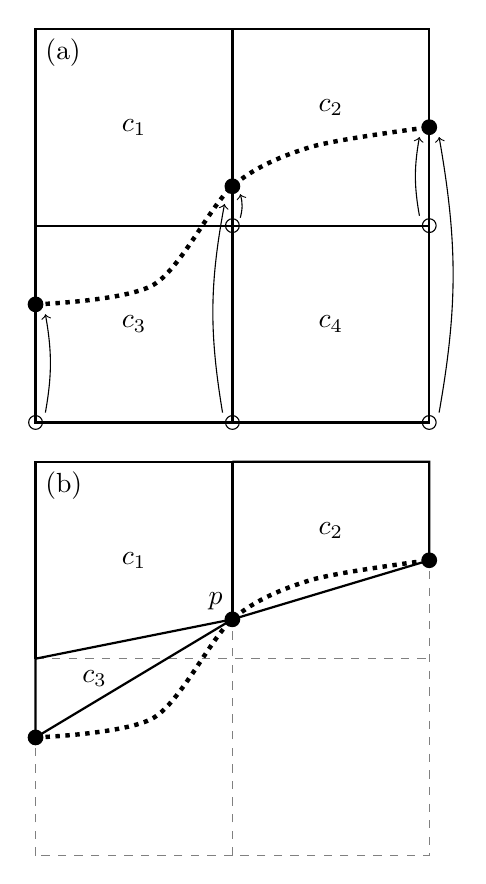
\begin{tikzpicture}[
  scale=0.25
]
\begin{scope}[shift={(0,22)}]
\draw [thick] (0,0) rectangle (20, 20);
\draw [thick] (10,0) -- (10,20);
\draw [thick] (0,10) -- (20,10);
\draw [dotted, ultra thick] plot [smooth] coordinates {(0,6) (6, 7) (10,12) (14,14) (20,15)};
\fill (0,6) circle [radius=0.4];
\fill (10,12) circle [radius=0.4];
\fill (20,15) circle [radius=0.4];
\draw (0,0) circle [radius=0.35];
\draw (10,0) circle [radius=0.35];
\draw (10,10) circle [radius=0.35];
\draw (20,0) circle [radius=0.35];
\draw (20,10) circle [radius=0.35];
\draw [->] (0.5,0.5) to [bend right=10] (0.5,5.5);
\draw [->] (9.5,0.5) to [bend left=10] (9.6,11.1);
\draw [->] (10.4,10.4) to [bend right=15] (10.4,11.6);
\draw [->] (19.5,10.5) to [bend left=10] (19.5,14.5);
\draw [->] (20.5,0.5) to [bend right=10] (20.5,14.5);
\node at (5,15) {$c_1$};
\node at (15,16) {$c_2$};
\node at (5,5) {$c_3$};
\node at (15,5) {$c_4$};

\node [below right] at (0,20) {(a)};

\draw [white] (20.6,0) rectangle (20.7,0);
\end{scope}

\draw [dashed, gray] (0,0) rectangle (20, 20);
\draw [dashed, gray] (10,0) -- (10,20);
\draw [dashed, gray] (0,10) -- (20,10);

\draw [thick] (0,6) -- (10,12) -- (0,10) -- (0,6);
\draw [thick] (0,10) -- (0,20) -- (10,20) -- (10,12);
\draw [thick] (10,20) -- (20,20) -- (20,15) -- (10,12);
\draw [dotted, ultra thick] plot [smooth] coordinates {(0,6) (6, 7) (10,12) (14,14) (20,15)};
\fill (0,6) circle [radius=0.4];
\fill (10,12) circle [radius=0.4] node [anchor=south east] {$p$};
\fill (20,15) circle [radius=0.4];
\node at (5,15) {$c_1$};
\node at (15,16.5) {$c_2$};
\node at (3,9) {$c_3$};

\node [below right] at (0,20) {(b)};
\end{tikzpicture}
\end{document}
